\documentclass[1p]{elsarticle_modified}
%\bibliographystyle{elsarticle-num}

%\usepackage[colorlinks]{hyperref}
%\usepackage{abbrmath_seonhwa} %\Abb, \Ascr, \Acal ,\Abf, \Afrak
\usepackage{amsfonts}
\usepackage{amssymb}
\usepackage{amsmath}
\usepackage{amsthm}
\usepackage{scalefnt}
\usepackage{amsbsy}
\usepackage{kotex}
\usepackage{caption}
\usepackage{subfig}
\usepackage{color}
\usepackage{graphicx}
\usepackage{xcolor} %% white, black, red, green, blue, cyan, magenta, yellow
\usepackage{float}
\usepackage{setspace}
\usepackage{hyperref}

\usepackage{tikz}
\usetikzlibrary{arrows}

\usepackage{multirow}
\usepackage{array} % fixed length table
\usepackage{hhline}

%%%%%%%%%%%%%%%%%%%%%
\makeatletter
\renewcommand*\env@matrix[1][\arraystretch]{%
	\edef\arraystretch{#1}%
	\hskip -\arraycolsep
	\let\@ifnextchar\new@ifnextchar
	\array{*\c@MaxMatrixCols c}}
\makeatother %https://tex.stackexchange.com/questions/14071/how-can-i-increase-the-line-spacing-in-a-matrix
%%%%%%%%%%%%%%%

\usepackage[normalem]{ulem}

\newcommand{\msout}[1]{\ifmmode\text{\sout{\ensuremath{#1}}}\else\sout{#1}\fi}
%SOURCE: \msout is \stkout macro in https://tex.stackexchange.com/questions/20609/strikeout-in-math-mode

\newcommand{\cancel}[1]{
	\ifmmode
	{\color{red}\msout{#1}}
	\else
	{\color{red}\sout{#1}}
	\fi
}

\newcommand{\add}[1]{
	{\color{blue}\uwave{#1}}
}

\newcommand{\replace}[2]{
	\ifmmode
	{\color{red}\msout{#1}}{\color{blue}\uwave{#2}}
	\else
	{\color{red}\sout{#1}}{\color{blue}\uwave{#2}}
	\fi
}

\newcommand{\Sol}{\mathcal{S}} %segment
\newcommand{\D}{D} %diagram
\newcommand{\A}{\mathcal{A}} %arc


%%%%%%%%%%%%%%%%%%%%%%%%%%%%%5 test

\def\sl{\operatorname{\textup{SL}}(2,\Cbb)}
\def\psl{\operatorname{\textup{PSL}}(2,\Cbb)}
\def\quan{\mkern 1mu \triangleright \mkern 1mu}

\theoremstyle{definition}
\newtheorem{thm}{Theorem}[section]
\newtheorem{prop}[thm]{Proposition}
\newtheorem{lem}[thm]{Lemma}
\newtheorem{ques}[thm]{Question}
\newtheorem{cor}[thm]{Corollary}
\newtheorem{defn}[thm]{Definition}
\newtheorem{exam}[thm]{Example}
\newtheorem{rmk}[thm]{Remark}
\newtheorem{alg}[thm]{Algorithm}

\newcommand{\I}{\sqrt{-1}}
\begin{document}

%\begin{frontmatter}
%
%\title{Boundary parabolic representations of knots up to 8 crossings}
%
%%% Group authors per affiliation:
%\author{Yunhi Cho} 
%\address{Department of Mathematics, University of Seoul, Seoul, Korea}
%\ead{yhcho@uos.ac.kr}
%
%
%\author{Seonhwa Kim} %\fnref{s_kim}}
%\address{Center for Geometry and Physics, Institute for Basic Science, Pohang, 37673, Korea}
%\ead{ryeona17@ibs.re.kr}
%
%\author{Hyuk Kim}
%\address{Department of Mathematical Sciences, Seoul National University, Seoul 08826, Korea}
%\ead{hyukkim@snu.ac.kr}
%
%\author{Seokbeom Yoon}
%\address{Department of Mathematical Sciences, Seoul National University, Seoul, 08826,  Korea}
%\ead{sbyoon15@snu.ac.kr}
%
%\begin{abstract}
%We find all boundary parabolic representation of knots up to 8 crossings.
%
%\end{abstract}
%\begin{keyword}
%    \MSC[2010] 57M25 
%\end{keyword}
%
%\end{frontmatter}

%\linenumbers
%\tableofcontents
%
\newcommand\colored[1]{\textcolor{white}{\rule[-0.35ex]{0.8em}{1.4ex}}\kern-0.8em\color{red} #1}%
%\newcommand\colored[1]{\textcolor{white}{ #1}\kern-2.17ex	\textcolor{white}{ #1}\kern-1.81ex	\textcolor{white}{ #1}\kern-2.15ex\color{red}#1	}

{\Large $\underline{12a_{0503}~(K12a_{0503})}$}

\setlength{\tabcolsep}{10pt}
\renewcommand{\arraystretch}{1.6}
\vspace{1cm}\begin{tabular}{m{100pt}>{\centering\arraybackslash}m{274pt}}
\multirow{5}{120pt}{
	\centering
	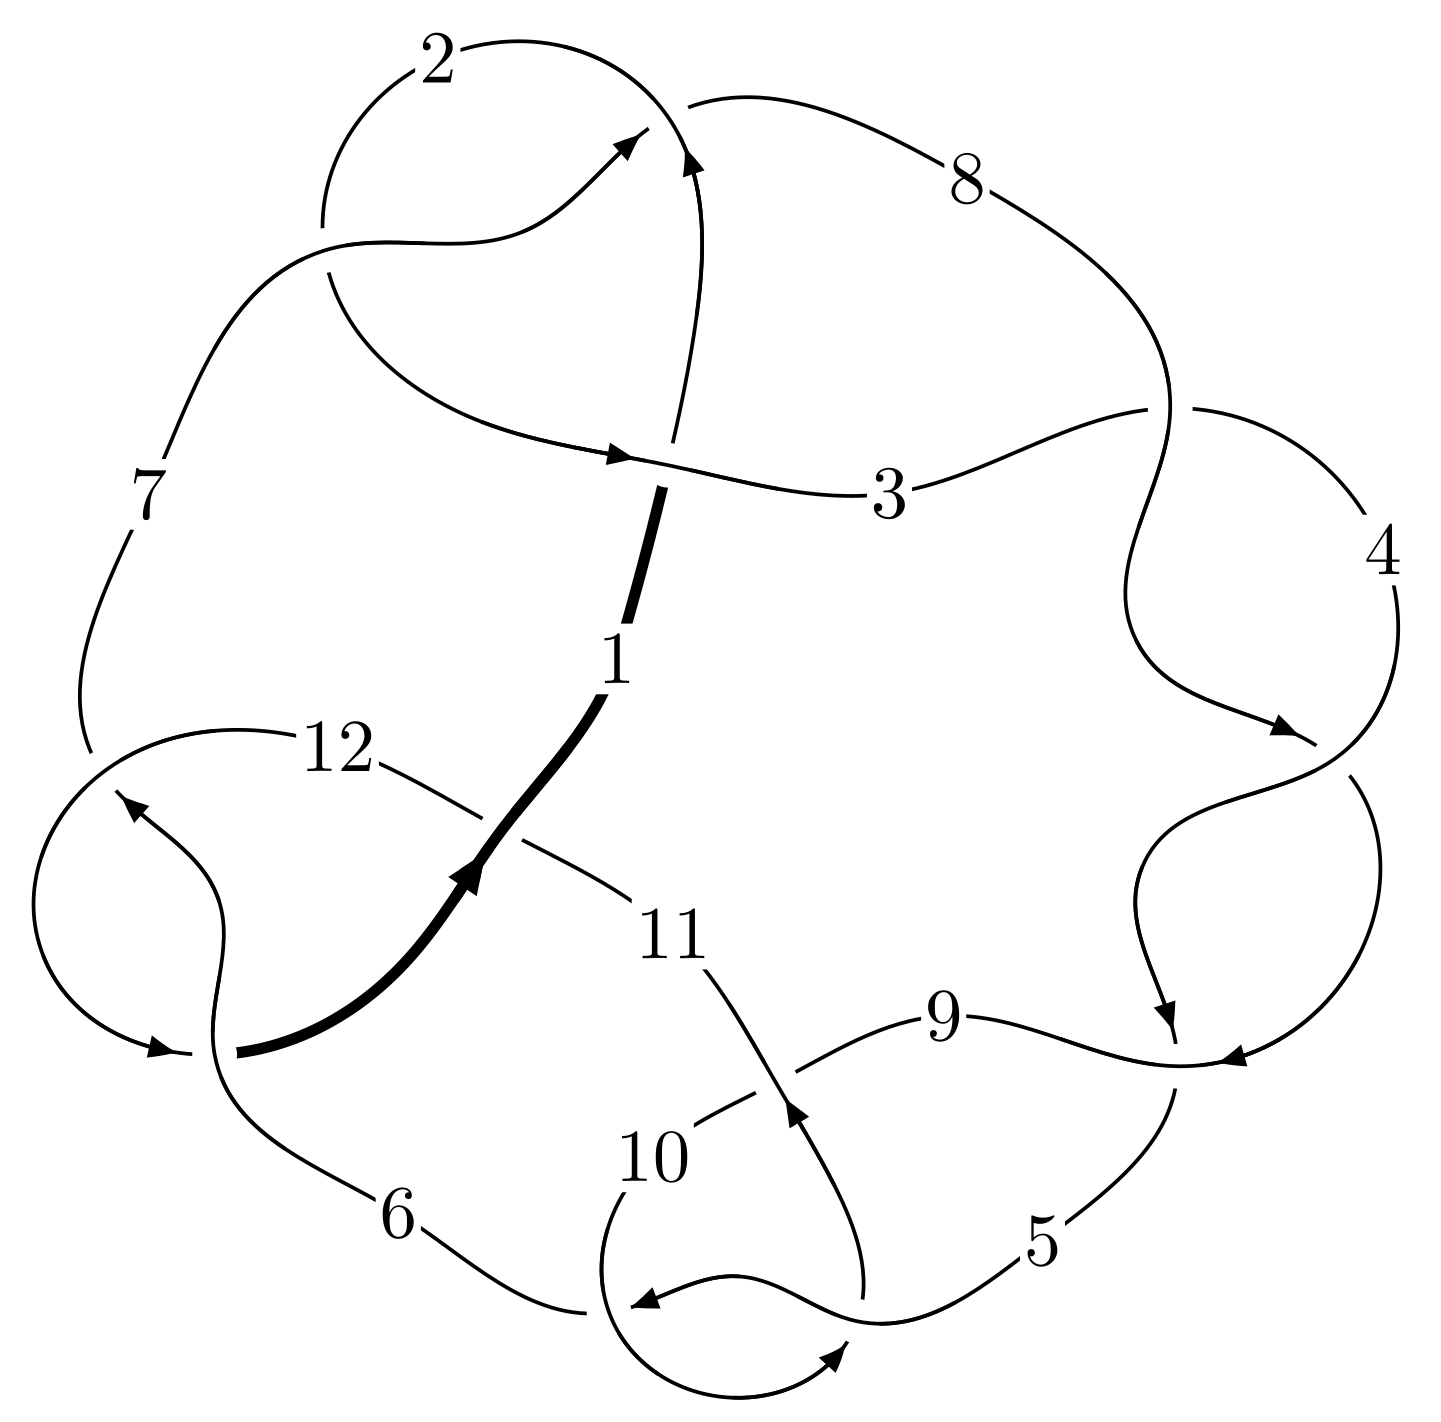
\includegraphics[width=112pt]{../../../GIT/diagram.site/Diagrams/png/1304_12a_0503.png}\\
\ \ \ A knot diagram\footnotemark}&
\allowdisplaybreaks
\textbf{Linearized knot diagam} \\
\cline{2-2}
 &
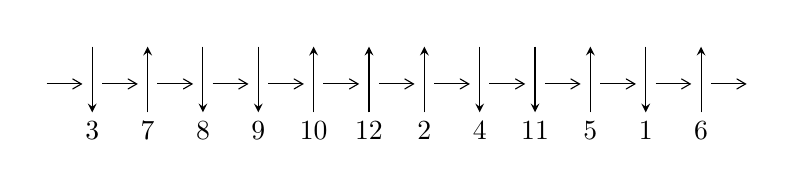
\begin{tikzpicture}[x=20pt, y=17pt]
	% nodes
	\node (C0) at (0, 0) {};
	\node (C1) at (1, 0) {};
	\node (C1U) at (1, +1) {};
	\node (C1D) at (1, -1) {3};

	\node (C2) at (2, 0) {};
	\node (C2U) at (2, +1) {};
	\node (C2D) at (2, -1) {7};

	\node (C3) at (3, 0) {};
	\node (C3U) at (3, +1) {};
	\node (C3D) at (3, -1) {8};

	\node (C4) at (4, 0) {};
	\node (C4U) at (4, +1) {};
	\node (C4D) at (4, -1) {9};

	\node (C5) at (5, 0) {};
	\node (C5U) at (5, +1) {};
	\node (C5D) at (5, -1) {10};

	\node (C6) at (6, 0) {};
	\node (C6U) at (6, +1) {};
	\node (C6D) at (6, -1) {12};

	\node (C7) at (7, 0) {};
	\node (C7U) at (7, +1) {};
	\node (C7D) at (7, -1) {2};

	\node (C8) at (8, 0) {};
	\node (C8U) at (8, +1) {};
	\node (C8D) at (8, -1) {4};

	\node (C9) at (9, 0) {};
	\node (C9U) at (9, +1) {};
	\node (C9D) at (9, -1) {11};

	\node (C10) at (10, 0) {};
	\node (C10U) at (10, +1) {};
	\node (C10D) at (10, -1) {5};

	\node (C11) at (11, 0) {};
	\node (C11U) at (11, +1) {};
	\node (C11D) at (11, -1) {1};

	\node (C12) at (12, 0) {};
	\node (C12U) at (12, +1) {};
	\node (C12D) at (12, -1) {6};
	\node (C13) at (13, 0) {};

	% arrows
	\draw[->,>={angle 60}]
	(C0) edge (C1) (C1) edge (C2) (C2) edge (C3) (C3) edge (C4) (C4) edge (C5) (C5) edge (C6) (C6) edge (C7) (C7) edge (C8) (C8) edge (C9) (C9) edge (C10) (C10) edge (C11) (C11) edge (C12) (C12) edge (C13) ;	\draw[->,>=stealth]
	(C1U) edge (C1D) (C2D) edge (C2U) (C3U) edge (C3D) (C4U) edge (C4D) (C5D) edge (C5U) (C6D) edge (C6U) (C7D) edge (C7U) (C8U) edge (C8D) (C9U) edge (C9D) (C10D) edge (C10U) (C11U) edge (C11D) (C12D) edge (C12U) ;
	\end{tikzpicture} \\
\hhline{~~} \\& 
\textbf{Solving Sequence} \\ \cline{2-2} 
 &
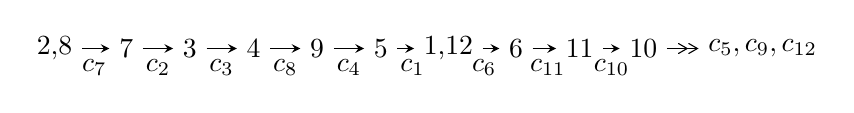
\begin{tikzpicture}[x=23pt, y=7pt]
	% node
	\node (A0) at (-1/8, 0) {2,8};
	\node (A1) at (1, 0) {7};
	\node (A2) at (2, 0) {3};
	\node (A3) at (3, 0) {4};
	\node (A4) at (4, 0) {9};
	\node (A5) at (5, 0) {5};
	\node (A6) at (97/16, 0) {1,12};
	\node (A7) at (57/8, 0) {6};
	\node (A8) at (65/8, 0) {11};
	\node (A9) at (73/8, 0) {10};
	\node (C1) at (1/2, -1) {$c_{7}$};
	\node (C2) at (3/2, -1) {$c_{2}$};
	\node (C3) at (5/2, -1) {$c_{3}$};
	\node (C4) at (7/2, -1) {$c_{8}$};
	\node (C5) at (9/2, -1) {$c_{4}$};
	\node (C6) at (11/2, -1) {$c_{1}$};
	\node (C7) at (53/8, -1) {$c_{6}$};
	\node (C8) at (61/8, -1) {$c_{11}$};
	\node (C9) at (69/8, -1) {$c_{10}$};
	\node (A10) at (11, 0) {$c_{5},c_{9},c_{12}$};

	% edge
	\draw[->,>=stealth]	
	(A0) edge (A1) (A1) edge (A2) (A2) edge (A3) (A3) edge (A4) (A4) edge (A5) (A5) edge (A6) (A6) edge (A7) (A7) edge (A8) (A8) edge (A9) ;
	\draw[->>,>={angle 60}]	
	(A9) edge (A10);
\end{tikzpicture} \\ 

\end{tabular} \\

\footnotetext{
The image of knot diagram is generated by the software ``\textbf{Draw programme}" developed by Andrew Bartholomew(\url{http://www.layer8.co.uk/maths/draw/index.htm\#Running-draw}), where we modified some parts for our purpose(\url{https://github.com/CATsTAILs/LinksPainter}).
}\phantom \\ \newline 
\centering \textbf{Ideals for irreducible components\footnotemark of $X_{\text{par}}$} 
 
\begin{align*}
I^u_{1}&=\langle 
- u^5-2 u^3+b+1,\;u^5+u^3+a-1,\;u^7+2 u^5+2 u^3- u^2- u-1\rangle \\
I^u_{2}&=\langle 
- u^{15}-5 u^{13}- u^{12}-12 u^{11}-4 u^{10}-15 u^9-8 u^8-10 u^7-8 u^6-2 u^5-5 u^4+u^3-2 u^2+b-1,\\
\phantom{I^u_{2}}&\phantom{= \langle  }u^{15}+2 u^{14}+5 u^{13}+9 u^{12}+12 u^{11}+19 u^{10}+15 u^9+19 u^8+10 u^7+8 u^6+2 u^5-2 u^4- u^2+a+2 u,\\
\phantom{I^u_{2}}&\phantom{= \langle  }u^{16}+u^{15}+5 u^{14}+5 u^{13}+12 u^{12}+12 u^{11}+15 u^{10}+15 u^9+10 u^8+10 u^7+2 u^6+2 u^5+u^2+1\rangle \\
I^u_{3}&=\langle 
- u^{15}+2 u^{14}-7 u^{13}+9 u^{12}-18 u^{11}+16 u^{10}-21 u^9+12 u^8-8 u^7+2 u^6+4 u^5- u^4+2 u^3+2 u^2+b-3 u+3,\\
\phantom{I^u_{3}}&\phantom{= \langle  }- u^{15}-3 u^{13}-2 u^{12}-2 u^{11}-6 u^{10}+3 u^9-6 u^8+4 u^7+4 u^4-2 u^3+2 u^2+2 a+u-1,\\
\phantom{I^u_{3}}&\phantom{= \langle  }u^{16}-2 u^{15}+7 u^{14}-10 u^{13}+18 u^{12}-20 u^{11}+21 u^{10}-18 u^9+8 u^8-4 u^7-4 u^6+4 u^5-2 u^4+3 u^2-3 u+2\rangle \\
I^u_{4}&=\langle 
u^{15}+3 u^{13}+4 u^{11}- u^9-4 u^7-4 u^5+u^3+b-1,\;- u^{15}-3 u^{13}-4 u^{11}+u^9+4 u^7+4 u^5-2 u^3+a+1,\\
\phantom{I^u_{4}}&\phantom{= \langle  }u^{16}+u^{15}+5 u^{14}+5 u^{13}+12 u^{12}+12 u^{11}+15 u^{10}+15 u^9+10 u^8+10 u^7+2 u^6+2 u^5+u^2+1\rangle \\
I^u_{5}&=\langle 
b+u-1,\;a- u+2,\;u^2- u+1\rangle \\
I^u_{6}&=\langle 
u^5- u^2 a+2 u^3- u^2+b- a+u-1,\;-2 u^5 a- u^5-4 u^3 a+u^4+2 u^2 a-2 u^3+a^2- a u+4 u^2+2 a-2 u+2,\\
\phantom{I^u_{6}}&\phantom{= \langle  }u^6+2 u^4- u^3+u^2- u-1\rangle \\
I^u_{7}&=\langle 
b- u-1,\;a+2 u+1,\;u^2+1\rangle \\
\\
\end{align*}
\raggedright * 7 irreducible components of $\dim_{\mathbb{C}}=0$, with total 71 representations.\\
\footnotetext{All coefficients of polynomials are rational numbers. But the coefficients are sometimes approximated in decimal forms when there is not enough margin.}
\newpage
\renewcommand{\arraystretch}{1}
\centering \section*{I. $I^u_{1}= \langle - u^5-2 u^3+b+1,\;u^5+u^3+a-1,\;u^7+2 u^5+2 u^3- u^2- u-1 \rangle$}
\flushleft \textbf{(i) Arc colorings}\\
\begin{tabular}{m{7pt} m{180pt} m{7pt} m{180pt} }
\flushright $a_{2}=$&$\begin{pmatrix}0\\u\end{pmatrix}$ \\
\flushright $a_{8}=$&$\begin{pmatrix}1\\0\end{pmatrix}$ \\
\flushright $a_{7}=$&$\begin{pmatrix}1\\u^2\end{pmatrix}$ \\
\flushright $a_{3}=$&$\begin{pmatrix}u\\u^3+u\end{pmatrix}$ \\
\flushright $a_{4}=$&$\begin{pmatrix}- u^3\\u^3+u\end{pmatrix}$ \\
\flushright $a_{9}=$&$\begin{pmatrix}- u^6- u^4+1\\u^6+2 u^4+u^2\end{pmatrix}$ \\
\flushright $a_{5}=$&$\begin{pmatrix}- u^5+u^4- u^3+u^2- u\\u^5- u^4+u^3-2 u^2-1\end{pmatrix}$ \\
\flushright $a_{1}=$&$\begin{pmatrix}u^3\\u^5+u^3+u\end{pmatrix}$ \\
\flushright $a_{12}=$&$\begin{pmatrix}- u^5- u^3+1\\u^5+2 u^3-1\end{pmatrix}$ \\
\flushright $a_{6}=$&$\begin{pmatrix}- u^6- u^4+u+1\\u^6+2 u^4+u^2- u\end{pmatrix}$ \\
\flushright $a_{11}=$&$\begin{pmatrix}- u^3+1\\u^3+u^2+u\end{pmatrix}$ \\
\flushright $a_{10}=$&$\begin{pmatrix}- u^6+u^5- u^4- u^2+1\\u^6- u^5+u^4- u^3+u^2\end{pmatrix}$\\&\end{tabular}
\flushleft \textbf{(ii) Obstruction class $= -1$}\\~\\
\flushleft \textbf{(iii) Cusp Shapes $= -6 u^6-6 u^4-6 u^2+6 u+6$}\\~\\
\newpage\renewcommand{\arraystretch}{1}
\flushleft \textbf{(iv) u-Polynomials at the component}\newline \\
\begin{tabular}{m{50pt}|m{274pt}}
Crossings & \hspace{64pt}u-Polynomials at each crossing \\
\hline $$\begin{aligned}c_{1},c_{9},c_{11}\end{aligned}$$&$\begin{aligned}
&u^7+4 u^6+8 u^5+6 u^4-5 u^2- u-1
\end{aligned}$\\
\hline $$\begin{aligned}c_{2},c_{5},c_{6}\\c_{7},c_{10},c_{12}\end{aligned}$$&$\begin{aligned}
&u^7+2 u^5+2 u^3+u^2- u+1
\end{aligned}$\\
\hline $$\begin{aligned}c_{3},c_{4},c_{8}\end{aligned}$$&$\begin{aligned}
&u^7-5 u^5-2 u^4+7 u^3+4 u^2+4
\end{aligned}$\\
\hline
\end{tabular}\\~\\
\newpage\renewcommand{\arraystretch}{1}
\flushleft \textbf{(v) Riley Polynomials at the component}\newline \\
\begin{tabular}{m{50pt}|m{274pt}}
Crossings & \hspace{64pt}Riley Polynomials at each crossing \\
\hline $$\begin{aligned}c_{1},c_{9},c_{11}\end{aligned}$$&$\begin{aligned}
&y^7+16 y^5+2 y^4+52 y^3-13 y^2-9 y-1
\end{aligned}$\\
\hline $$\begin{aligned}c_{2},c_{5},c_{6}\\c_{7},c_{10},c_{12}\end{aligned}$$&$\begin{aligned}
&y^7+4 y^6+8 y^5+6 y^4-5 y^2- y-1
\end{aligned}$\\
\hline $$\begin{aligned}c_{3},c_{4},c_{8}\end{aligned}$$&$\begin{aligned}
&y^7-10 y^6+39 y^5-74 y^4+65 y^3-32 y-16
\end{aligned}$\\
\hline
\end{tabular}\\~\\
\newpage\flushleft \textbf{(vi) Complex Volumes and Cusp Shapes}
$$\begin{array}{c|c|c}  
\text{Solutions to }I^u_{1}& \I (\text{vol} + \sqrt{-1}CS) & \text{Cusp shape}\\
 \hline 
\begin{aligned}
u &= \phantom{-}0.863824\phantom{ +0.000000I} \\
a &= -0.125557\phantom{ +0.000000I} \\
b &= \phantom{-}0.770135\phantom{ +0.000000I}\end{aligned}
 & -4.43886\phantom{ +0.000000I} & \phantom{-}0.872100\phantom{ +0.000000I} \\ \hline\begin{aligned}
u &= -0.506221 + 1.104710 I \\
a &= \phantom{-}1.49617 + 1.94571 I \\
b &= \phantom{-}0.22746 - 2.44461 I\end{aligned}
 & -5.20269 - 11.20360 I & -5.65627 + 10.71805 I \\ \hline\begin{aligned}
u &= -0.506221 - 1.104710 I \\
a &= \phantom{-}1.49617 - 1.94571 I \\
b &= \phantom{-}0.22746 + 2.44461 I\end{aligned}
 & -5.20269 + 11.20360 I & -5.65627 - 10.71805 I \\ \hline\begin{aligned}
u &= -0.426442 + 0.491723 I \\
a &= \phantom{-}0.719469 - 0.043211 I \\
b &= -0.487688 + 0.192580 I\end{aligned}
 & \phantom{-}0.805836 - 1.099860 I & \phantom{-}4.64625 + 4.74954 I \\ \hline\begin{aligned}
u &= -0.426442 - 0.491723 I \\
a &= \phantom{-}0.719469 + 0.043211 I \\
b &= -0.487688 - 0.192580 I\end{aligned}
 & \phantom{-}0.805836 + 1.099860 I & \phantom{-}4.64625 - 4.74954 I \\ \hline\begin{aligned}
u &= \phantom{-}0.500751 + 1.264820 I \\
a &= -1.15286 + 2.51108 I \\
b &= -1.12484 - 3.58304 I\end{aligned}
 & -15.5903 + 14.7635 I & -8.42603 - 8.80481 I \\ \hline\begin{aligned}
u &= \phantom{-}0.500751 - 1.264820 I \\
a &= -1.15286 - 2.51108 I \\
b &= -1.12484 + 3.58304 I\end{aligned}
 & -15.5903 - 14.7635 I & -8.42603 + 8.80481 I\\
 \hline 
 \end{array}$$\newpage\newpage\renewcommand{\arraystretch}{1}
\centering \section*{II. $I^u_{2}= \langle - u^{15}-5 u^{13}+\cdots+b-1,\;u^{15}+2 u^{14}+\cdots+a+2 u,\;u^{16}+u^{15}+\cdots+u^2+1 \rangle$}
\flushleft \textbf{(i) Arc colorings}\\
\begin{tabular}{m{7pt} m{180pt} m{7pt} m{180pt} }
\flushright $a_{2}=$&$\begin{pmatrix}0\\u\end{pmatrix}$ \\
\flushright $a_{8}=$&$\begin{pmatrix}1\\0\end{pmatrix}$ \\
\flushright $a_{7}=$&$\begin{pmatrix}1\\u^2\end{pmatrix}$ \\
\flushright $a_{3}=$&$\begin{pmatrix}u\\u^3+u\end{pmatrix}$ \\
\flushright $a_{4}=$&$\begin{pmatrix}- u^3\\u^3+u\end{pmatrix}$ \\
\flushright $a_{9}=$&$\begin{pmatrix}- u^6- u^4+1\\u^6+2 u^4+u^2\end{pmatrix}$ \\
\flushright $a_{5}=$&$\begin{pmatrix}u^9+2 u^7+u^5-2 u^3- u\\- u^9-3 u^7-3 u^5+u\end{pmatrix}$ \\
\flushright $a_{1}=$&$\begin{pmatrix}u^3\\u^5+u^3+u\end{pmatrix}$ \\
\flushright $a_{12}=$&$\begin{pmatrix}- u^{15}-2 u^{14}+\cdots+u^2-2 u\\u^{15}+5 u^{13}+\cdots+2 u^2+1\end{pmatrix}$ \\
\flushright $a_{6}=$&$\begin{pmatrix}u^{15}+3 u^{13}+3 u^{11}-3 u^9-6 u^7-2 u^5+3 u^3+u-1\\u^{11}+3 u^9+4 u^7+u^5- u^3- u\end{pmatrix}$ \\
\flushright $a_{11}=$&$\begin{pmatrix}- u^{15}-2 u^{14}+\cdots+u^4- u\\u^8+2 u^6+2 u^4\end{pmatrix}$ \\
\flushright $a_{10}=$&$\begin{pmatrix}- u^{15}-2 u^{14}+\cdots- u^2- u\\- u^{10}-2 u^8- u^6+2 u^4+u^2\end{pmatrix}$\\&\end{tabular}
\flushleft \textbf{(ii) Obstruction class $= -1$}\\~\\
\flushleft \textbf{(iii) Cusp Shapes $= -4 u^{14}-4 u^{13}-16 u^{12}-20 u^{11}-32 u^{10}-44 u^9-28 u^8-44 u^7-12 u^6-12 u^5+4 u^4+12 u^3-4 u^2+4 u-6$}\\~\\
\newpage\renewcommand{\arraystretch}{1}
\flushleft \textbf{(iv) u-Polynomials at the component}\newline \\
\begin{tabular}{m{50pt}|m{274pt}}
Crossings & \hspace{64pt}u-Polynomials at each crossing \\
\hline $$\begin{aligned}c_{1},c_{9}\end{aligned}$$&$\begin{aligned}
&u^{16}+9 u^{15}+\cdots+2 u+1
\end{aligned}$\\
\hline $$\begin{aligned}c_{2},c_{5},c_{7}\\c_{10}\end{aligned}$$&$\begin{aligned}
&u^{16}- u^{15}+\cdots+u^2+1
\end{aligned}$\\
\hline $$\begin{aligned}c_{3},c_{4},c_{8}\end{aligned}$$&$\begin{aligned}
&u^{16}-2 u^{15}+\cdots- u+2
\end{aligned}$\\
\hline $$\begin{aligned}c_{6},c_{12}\end{aligned}$$&$\begin{aligned}
&u^{16}+2 u^{15}+\cdots+3 u+2
\end{aligned}$\\
\hline $$\begin{aligned}c_{11}\end{aligned}$$&$\begin{aligned}
&u^{16}+10 u^{15}+\cdots+3 u+4
\end{aligned}$\\
\hline
\end{tabular}\\~\\
\newpage\renewcommand{\arraystretch}{1}
\flushleft \textbf{(v) Riley Polynomials at the component}\newline \\
\begin{tabular}{m{50pt}|m{274pt}}
Crossings & \hspace{64pt}Riley Polynomials at each crossing \\
\hline $$\begin{aligned}c_{1},c_{9}\end{aligned}$$&$\begin{aligned}
&y^{16}-3 y^{15}+\cdots-2 y+1
\end{aligned}$\\
\hline $$\begin{aligned}c_{2},c_{5},c_{7}\\c_{10}\end{aligned}$$&$\begin{aligned}
&y^{16}+9 y^{15}+\cdots+2 y+1
\end{aligned}$\\
\hline $$\begin{aligned}c_{3},c_{4},c_{8}\end{aligned}$$&$\begin{aligned}
&y^{16}-18 y^{15}+\cdots+19 y+4
\end{aligned}$\\
\hline $$\begin{aligned}c_{6},c_{12}\end{aligned}$$&$\begin{aligned}
&y^{16}+10 y^{15}+\cdots+3 y+4
\end{aligned}$\\
\hline $$\begin{aligned}c_{11}\end{aligned}$$&$\begin{aligned}
&y^{16}-10 y^{15}+\cdots- y+16
\end{aligned}$\\
\hline
\end{tabular}\\~\\
\newpage\flushleft \textbf{(vi) Complex Volumes and Cusp Shapes}
$$\begin{array}{c|c|c}  
\text{Solutions to }I^u_{2}& \I (\text{vol} + \sqrt{-1}CS) & \text{Cusp shape}\\
 \hline 
\begin{aligned}
u &= -0.892953 + 0.035958 I \\
a &= -0.652536 + 1.200890 I \\
b &= \phantom{-}0.02318 + 2.24381 I\end{aligned}
 & -8.19036 + 4.73480 I & -2.47201 - 3.02289 I \\ \hline\begin{aligned}
u &= -0.892953 - 0.035958 I \\
a &= -0.652536 - 1.200890 I \\
b &= \phantom{-}0.02318 - 2.24381 I\end{aligned}
 & -8.19036 - 4.73480 I & -2.47201 + 3.02289 I \\ \hline\begin{aligned}
u &= -0.458901 + 0.734878 I \\
a &= -0.104273 - 0.435411 I \\
b &= \phantom{-}0.247757 + 0.757374 I\end{aligned}
 & \phantom{-}0.85997 - 1.95072 I & \phantom{-}3.06114 + 4.17042 I \\ \hline\begin{aligned}
u &= -0.458901 - 0.734878 I \\
a &= -0.104273 + 0.435411 I \\
b &= \phantom{-}0.247757 - 0.757374 I\end{aligned}
 & \phantom{-}0.85997 + 1.95072 I & \phantom{-}3.06114 - 4.17042 I \\ \hline\begin{aligned}
u &= -0.379593 + 1.079580 I \\
a &= -0.56037 - 2.03187 I \\
b &= -1.36347 + 1.32712 I\end{aligned}
 & -7.04324 - 3.37292 I & -8.93248 + 5.20888 I \\ \hline\begin{aligned}
u &= -0.379593 - 1.079580 I \\
a &= -0.56037 + 2.03187 I \\
b &= -1.36347 - 1.32712 I\end{aligned}
 & -7.04324 + 3.37292 I & -8.93248 - 5.20888 I \\ \hline\begin{aligned}
u &= \phantom{-}0.469252 + 1.053160 I \\
a &= -0.371270 - 0.561834 I \\
b &= \phantom{-}0.161095 + 0.362888 I\end{aligned}
 & -2.68724 + 6.60937 I & -2.51664 - 7.40663 I \\ \hline\begin{aligned}
u &= \phantom{-}0.469252 - 1.053160 I \\
a &= -0.371270 + 0.561834 I \\
b &= \phantom{-}0.161095 - 0.362888 I\end{aligned}
 & -2.68724 - 6.60937 I & -2.51664 + 7.40663 I \\ \hline\begin{aligned}
u &= \phantom{-}0.190701 + 0.810384 I \\
a &= \phantom{-}0.33485 - 2.32194 I \\
b &= \phantom{-}0.569648 + 0.391218 I\end{aligned}
 & -3.86698 + 1.08438 I & -3.75949 - 5.90127 I \\ \hline\begin{aligned}
u &= \phantom{-}0.190701 - 0.810384 I \\
a &= \phantom{-}0.33485 + 2.32194 I \\
b &= \phantom{-}0.569648 - 0.391218 I\end{aligned}
 & -3.86698 - 1.08438 I & -3.75949 + 5.90127 I\\
 \hline 
 \end{array}$$\newpage$$\begin{array}{c|c|c}  
\text{Solutions to }I^u_{2}& \I (\text{vol} + \sqrt{-1}CS) & \text{Cusp shape}\\
 \hline 
\begin{aligned}
u &= -0.487539 + 1.254270 I \\
a &= \phantom{-}0.652357 - 0.643137 I \\
b &= -0.736189 + 0.110556 I\end{aligned}
 & -11.8837 - 9.6751 I & -5.50822 + 5.97678 I \\ \hline\begin{aligned}
u &= -0.487539 - 1.254270 I \\
a &= \phantom{-}0.652357 + 0.643137 I \\
b &= -0.736189 - 0.110556 I\end{aligned}
 & -11.8837 + 9.6751 I & -5.50822 - 5.97678 I \\ \hline\begin{aligned}
u &= \phantom{-}0.469746 + 1.263010 I \\
a &= \phantom{-}0.70256 - 1.98263 I \\
b &= \phantom{-}1.83074 + 2.27175 I\end{aligned}
 & -16.0195 + 4.8597 I & -9.14726 - 3.11789 I \\ \hline\begin{aligned}
u &= \phantom{-}0.469746 - 1.263010 I \\
a &= \phantom{-}0.70256 + 1.98263 I \\
b &= \phantom{-}1.83074 - 2.27175 I\end{aligned}
 & -16.0195 - 4.8597 I & -9.14726 + 3.11789 I \\ \hline\begin{aligned}
u &= \phantom{-}0.589289 + 0.270476 I \\
a &= \phantom{-}0.998682 + 0.324734 I \\
b &= -0.232766 + 1.375450 I\end{aligned}
 & -0.51702 - 2.45923 I & \phantom{-}1.27496 + 3.25382 I \\ \hline\begin{aligned}
u &= \phantom{-}0.589289 - 0.270476 I \\
a &= \phantom{-}0.998682 - 0.324734 I \\
b &= -0.232766 - 1.375450 I\end{aligned}
 & -0.51702 + 2.45923 I & \phantom{-}1.27496 - 3.25382 I\\
 \hline 
 \end{array}$$\newpage\newpage\renewcommand{\arraystretch}{1}
\centering \section*{III. $I^u_{3}= \langle - u^{15}+2 u^{14}+\cdots+b+3,\;- u^{15}-3 u^{13}+\cdots+2 a-1,\;u^{16}-2 u^{15}+\cdots-3 u+2 \rangle$}
\flushleft \textbf{(i) Arc colorings}\\
\begin{tabular}{m{7pt} m{180pt} m{7pt} m{180pt} }
\flushright $a_{2}=$&$\begin{pmatrix}0\\u\end{pmatrix}$ \\
\flushright $a_{8}=$&$\begin{pmatrix}1\\0\end{pmatrix}$ \\
\flushright $a_{7}=$&$\begin{pmatrix}1\\u^2\end{pmatrix}$ \\
\flushright $a_{3}=$&$\begin{pmatrix}u\\u^3+u\end{pmatrix}$ \\
\flushright $a_{4}=$&$\begin{pmatrix}- u^3\\u^3+u\end{pmatrix}$ \\
\flushright $a_{9}=$&$\begin{pmatrix}- u^6- u^4+1\\u^6+2 u^4+u^2\end{pmatrix}$ \\
\flushright $a_{5}=$&$\begin{pmatrix}u^9+2 u^7+u^5-2 u^3- u\\- u^9-3 u^7-3 u^5+u\end{pmatrix}$ \\
\flushright $a_{1}=$&$\begin{pmatrix}u^3\\u^5+u^3+u\end{pmatrix}$ \\
\flushright $a_{12}=$&$\begin{pmatrix}\frac{1}{2} u^{15}+\frac{3}{2} u^{13}+\cdots-\frac{1}{2} u+\frac{1}{2}\\u^{15}-2 u^{14}+\cdots+3 u-3\end{pmatrix}$ \\
\flushright $a_{6}=$&$\begin{pmatrix}-\frac{1}{2} u^{15}+2 u^{14}+\cdots-\frac{3}{2} u+\frac{3}{2}\\u^{15}-2 u^{14}+\cdots+2 u-1\end{pmatrix}$ \\
\flushright $a_{11}=$&$\begin{pmatrix}\frac{1}{2} u^{15}-2 u^{14}+\cdots+\frac{5}{2} u-\frac{3}{2}\\- u^{15}+2 u^{14}+\cdots-2 u+1\end{pmatrix}$ \\
\flushright $a_{10}=$&$\begin{pmatrix}-\frac{1}{2} u^{15}-\frac{3}{2} u^{13}+\cdots+\frac{1}{2} u+\frac{1}{2}\\- u^{15}+2 u^{14}+\cdots-2 u+3\end{pmatrix}$\\&\end{tabular}
\flushleft \textbf{(ii) Obstruction class $= -1$}\\~\\
\flushleft \textbf{(iii) Cusp Shapes $= 4 u^{13}+16 u^{11}+24 u^9+4 u^7-20 u^5-12 u^3+4 u-6$}\\~\\
\newpage\renewcommand{\arraystretch}{1}
\flushleft \textbf{(iv) u-Polynomials at the component}\newline \\
\begin{tabular}{m{50pt}|m{274pt}}
Crossings & \hspace{64pt}u-Polynomials at each crossing \\
\hline $$\begin{aligned}c_{1}\end{aligned}$$&$\begin{aligned}
&u^{16}+10 u^{15}+\cdots+3 u+4
\end{aligned}$\\
\hline $$\begin{aligned}c_{2},c_{7}\end{aligned}$$&$\begin{aligned}
&u^{16}+2 u^{15}+\cdots+3 u+2
\end{aligned}$\\
\hline $$\begin{aligned}c_{3},c_{4},c_{8}\end{aligned}$$&$\begin{aligned}
&u^{16}-2 u^{15}+\cdots- u+2
\end{aligned}$\\
\hline $$\begin{aligned}c_{5},c_{6},c_{10}\\c_{12}\end{aligned}$$&$\begin{aligned}
&u^{16}- u^{15}+\cdots+u^2+1
\end{aligned}$\\
\hline $$\begin{aligned}c_{9},c_{11}\end{aligned}$$&$\begin{aligned}
&u^{16}+9 u^{15}+\cdots+2 u+1
\end{aligned}$\\
\hline
\end{tabular}\\~\\
\newpage\renewcommand{\arraystretch}{1}
\flushleft \textbf{(v) Riley Polynomials at the component}\newline \\
\begin{tabular}{m{50pt}|m{274pt}}
Crossings & \hspace{64pt}Riley Polynomials at each crossing \\
\hline $$\begin{aligned}c_{1}\end{aligned}$$&$\begin{aligned}
&y^{16}-10 y^{15}+\cdots- y+16
\end{aligned}$\\
\hline $$\begin{aligned}c_{2},c_{7}\end{aligned}$$&$\begin{aligned}
&y^{16}+10 y^{15}+\cdots+3 y+4
\end{aligned}$\\
\hline $$\begin{aligned}c_{3},c_{4},c_{8}\end{aligned}$$&$\begin{aligned}
&y^{16}-18 y^{15}+\cdots+19 y+4
\end{aligned}$\\
\hline $$\begin{aligned}c_{5},c_{6},c_{10}\\c_{12}\end{aligned}$$&$\begin{aligned}
&y^{16}+9 y^{15}+\cdots+2 y+1
\end{aligned}$\\
\hline $$\begin{aligned}c_{9},c_{11}\end{aligned}$$&$\begin{aligned}
&y^{16}-3 y^{15}+\cdots-2 y+1
\end{aligned}$\\
\hline
\end{tabular}\\~\\
\newpage\flushleft \textbf{(vi) Complex Volumes and Cusp Shapes}
$$\begin{array}{c|c|c}  
\text{Solutions to }I^u_{3}& \I (\text{vol} + \sqrt{-1}CS) & \text{Cusp shape}\\
 \hline 
\begin{aligned}
u &= -0.402991 + 0.968083 I \\
a &= \phantom{-}0.222795 - 0.609931 I \\
b &= -0.059233 + 0.569202 I\end{aligned}
 & -0.51702 - 2.45923 I & \phantom{-}1.27496 + 3.25382 I \\ \hline\begin{aligned}
u &= -0.402991 - 0.968083 I \\
a &= \phantom{-}0.222795 + 0.609931 I \\
b &= -0.059233 - 0.569202 I\end{aligned}
 & -0.51702 + 2.45923 I & \phantom{-}1.27496 - 3.25382 I \\ \hline\begin{aligned}
u &= \phantom{-}0.921586 + 0.049492 I \\
a &= \phantom{-}0.594426 + 1.196160 I \\
b &= -0.09325 + 2.32148 I\end{aligned}
 & -11.8837 - 9.6751 I & -5.50822 + 5.97678 I \\ \hline\begin{aligned}
u &= \phantom{-}0.921586 - 0.049492 I \\
a &= \phantom{-}0.594426 - 1.196160 I \\
b &= -0.09325 - 2.32148 I\end{aligned}
 & -11.8837 + 9.6751 I & -5.50822 - 5.97678 I \\ \hline\begin{aligned}
u &= \phantom{-}0.059705 + 1.152710 I \\
a &= \phantom{-}0.23551 - 1.67559 I \\
b &= \phantom{-}0.10924 + 1.44246 I\end{aligned}
 & -3.86698 - 1.08438 I & -3.75949 + 5.90127 I \\ \hline\begin{aligned}
u &= \phantom{-}0.059705 - 1.152710 I \\
a &= \phantom{-}0.23551 + 1.67559 I \\
b &= \phantom{-}0.10924 - 1.44246 I\end{aligned}
 & -3.86698 + 1.08438 I & -3.75949 - 5.90127 I \\ \hline\begin{aligned}
u &= -0.270509 + 1.207500 I \\
a &= -0.55626 - 1.86816 I \\
b &= -0.82968 + 1.87098 I\end{aligned}
 & -7.04324 + 3.37292 I & -8.93248 - 5.20888 I \\ \hline\begin{aligned}
u &= -0.270509 - 1.207500 I \\
a &= -0.55626 + 1.86816 I \\
b &= -0.82968 - 1.87098 I\end{aligned}
 & -7.04324 - 3.37292 I & -8.93248 + 5.20888 I \\ \hline\begin{aligned}
u &= -0.724264 + 0.230405 I \\
a &= -0.784571 + 0.654294 I \\
b &= \phantom{-}0.31772 + 1.62349 I\end{aligned}
 & -2.68724 + 6.60937 I & -2.51664 - 7.40663 I \\ \hline\begin{aligned}
u &= -0.724264 - 0.230405 I \\
a &= -0.784571 - 0.654294 I \\
b &= \phantom{-}0.31772 - 1.62349 I\end{aligned}
 & -2.68724 - 6.60937 I & -2.51664 + 7.40663 I\\
 \hline 
 \end{array}$$\newpage$$\begin{array}{c|c|c}  
\text{Solutions to }I^u_{3}& \I (\text{vol} + \sqrt{-1}CS) & \text{Cusp shape}\\
 \hline 
\begin{aligned}
u &= \phantom{-}0.507077 + 0.543596 I \\
a &= \phantom{-}0.458679 - 0.248786 I \\
b &= -0.339347 + 0.997289 I\end{aligned}
 & \phantom{-}0.85997 - 1.95072 I & \phantom{-}3.06114 + 4.17042 I \\ \hline\begin{aligned}
u &= \phantom{-}0.507077 - 0.543596 I \\
a &= \phantom{-}0.458679 + 0.248786 I \\
b &= -0.339347 - 0.997289 I\end{aligned}
 & \phantom{-}0.85997 + 1.95072 I & \phantom{-}3.06114 - 4.17042 I \\ \hline\begin{aligned}
u &= \phantom{-}0.465530 + 1.245910 I \\
a &= -0.629795 - 0.668340 I \\
b &= \phantom{-}0.723472 + 0.198002 I\end{aligned}
 & -8.19036 + 4.73480 I & -2.47201 - 3.02289 I \\ \hline\begin{aligned}
u &= \phantom{-}0.465530 - 1.245910 I \\
a &= -0.629795 + 0.668340 I \\
b &= \phantom{-}0.723472 - 0.198002 I\end{aligned}
 & -8.19036 - 4.73480 I & -2.47201 + 3.02289 I \\ \hline\begin{aligned}
u &= \phantom{-}0.443866 + 1.287090 I \\
a &= \phantom{-}0.70921 - 1.95738 I \\
b &= \phantom{-}1.67108 + 2.40426 I\end{aligned}
 & -16.0195 - 4.8597 I & -9.14726 + 3.11789 I \\ \hline\begin{aligned}
u &= \phantom{-}0.443866 - 1.287090 I \\
a &= \phantom{-}0.70921 + 1.95738 I \\
b &= \phantom{-}1.67108 - 2.40426 I\end{aligned}
 & -16.0195 + 4.8597 I & -9.14726 - 3.11789 I\\
 \hline 
 \end{array}$$\newpage\newpage\renewcommand{\arraystretch}{1}
\centering \section*{IV. $I^u_{4}= \langle u^{15}+3 u^{13}+4 u^{11}- u^9-4 u^7-4 u^5+u^3+b-1,\;- u^{15}-3 u^{13}+\cdots+a+1,\;u^{16}+u^{15}+\cdots+u^2+1 \rangle$}
\flushleft \textbf{(i) Arc colorings}\\
\begin{tabular}{m{7pt} m{180pt} m{7pt} m{180pt} }
\flushright $a_{2}=$&$\begin{pmatrix}0\\u\end{pmatrix}$ \\
\flushright $a_{8}=$&$\begin{pmatrix}1\\0\end{pmatrix}$ \\
\flushright $a_{7}=$&$\begin{pmatrix}1\\u^2\end{pmatrix}$ \\
\flushright $a_{3}=$&$\begin{pmatrix}u\\u^3+u\end{pmatrix}$ \\
\flushright $a_{4}=$&$\begin{pmatrix}- u^3\\u^3+u\end{pmatrix}$ \\
\flushright $a_{9}=$&$\begin{pmatrix}- u^6- u^4+1\\u^6+2 u^4+u^2\end{pmatrix}$ \\
\flushright $a_{5}=$&$\begin{pmatrix}u^9+2 u^7+u^5-2 u^3- u\\- u^9-3 u^7-3 u^5+u\end{pmatrix}$ \\
\flushright $a_{1}=$&$\begin{pmatrix}u^3\\u^5+u^3+u\end{pmatrix}$ \\
\flushright $a_{12}=$&$\begin{pmatrix}u^{15}+3 u^{13}+4 u^{11}- u^9-4 u^7-4 u^5+2 u^3-1\\- u^{15}-3 u^{13}-4 u^{11}+u^9+4 u^7+4 u^5- u^3+1\end{pmatrix}$ \\
\flushright $a_{6}=$&$\begin{pmatrix}- u^{15}-2 u^{14}+\cdots- u^2- u\\u^{15}+2 u^{14}+\cdots+u+1\end{pmatrix}$ \\
\flushright $a_{11}=$&$\begin{pmatrix}u^{15}+3 u^{13}+4 u^{11}- u^9-4 u^7-3 u^5+2 u^3-1\\- u^{15}-3 u^{13}-4 u^{11}+u^9+5 u^7+5 u^5+1\end{pmatrix}$ \\
\flushright $a_{10}=$&$\begin{pmatrix}u^{15}+3 u^{13}+4 u^{11}- u^{10}- u^9-3 u^8-4 u^7-4 u^6-4 u^5- u^4+u^3+u^2- u\\2 u^{13}+8 u^{11}+\cdots- u+2\end{pmatrix}$\\&\end{tabular}
\flushleft \textbf{(ii) Obstruction class $= -1$}\\~\\
\flushleft \textbf{(iii) Cusp Shapes $= -4 u^{14}-4 u^{13}-16 u^{12}-20 u^{11}-32 u^{10}-44 u^9-28 u^8-44 u^7-12 u^6-12 u^5+4 u^4+12 u^3-4 u^2+4 u-6$}\\~\\
\newpage\renewcommand{\arraystretch}{1}
\flushleft \textbf{(iv) u-Polynomials at the component}\newline \\
\begin{tabular}{m{50pt}|m{274pt}}
Crossings & \hspace{64pt}u-Polynomials at each crossing \\
\hline $$\begin{aligned}c_{1},c_{11}\end{aligned}$$&$\begin{aligned}
&u^{16}+9 u^{15}+\cdots+2 u+1
\end{aligned}$\\
\hline $$\begin{aligned}c_{2},c_{6},c_{7}\\c_{12}\end{aligned}$$&$\begin{aligned}
&u^{16}- u^{15}+\cdots+u^2+1
\end{aligned}$\\
\hline $$\begin{aligned}c_{3},c_{4},c_{8}\end{aligned}$$&$\begin{aligned}
&u^{16}-2 u^{15}+\cdots- u+2
\end{aligned}$\\
\hline $$\begin{aligned}c_{5},c_{10}\end{aligned}$$&$\begin{aligned}
&u^{16}+2 u^{15}+\cdots+3 u+2
\end{aligned}$\\
\hline $$\begin{aligned}c_{9}\end{aligned}$$&$\begin{aligned}
&u^{16}+10 u^{15}+\cdots+3 u+4
\end{aligned}$\\
\hline
\end{tabular}\\~\\
\newpage\renewcommand{\arraystretch}{1}
\flushleft \textbf{(v) Riley Polynomials at the component}\newline \\
\begin{tabular}{m{50pt}|m{274pt}}
Crossings & \hspace{64pt}Riley Polynomials at each crossing \\
\hline $$\begin{aligned}c_{1},c_{11}\end{aligned}$$&$\begin{aligned}
&y^{16}-3 y^{15}+\cdots-2 y+1
\end{aligned}$\\
\hline $$\begin{aligned}c_{2},c_{6},c_{7}\\c_{12}\end{aligned}$$&$\begin{aligned}
&y^{16}+9 y^{15}+\cdots+2 y+1
\end{aligned}$\\
\hline $$\begin{aligned}c_{3},c_{4},c_{8}\end{aligned}$$&$\begin{aligned}
&y^{16}-18 y^{15}+\cdots+19 y+4
\end{aligned}$\\
\hline $$\begin{aligned}c_{5},c_{10}\end{aligned}$$&$\begin{aligned}
&y^{16}+10 y^{15}+\cdots+3 y+4
\end{aligned}$\\
\hline $$\begin{aligned}c_{9}\end{aligned}$$&$\begin{aligned}
&y^{16}-10 y^{15}+\cdots- y+16
\end{aligned}$\\
\hline
\end{tabular}\\~\\
\newpage\flushleft \textbf{(vi) Complex Volumes and Cusp Shapes}
$$\begin{array}{c|c|c}  
\text{Solutions to }I^u_{4}& \I (\text{vol} + \sqrt{-1}CS) & \text{Cusp shape}\\
 \hline 
\begin{aligned}
u &= -0.892953 + 0.035958 I \\
a &= \phantom{-}0.1015470 + 0.0314751 I \\
b &= -0.810093 + 0.054493 I\end{aligned}
 & -8.19036 + 4.73480 I & -2.47201 - 3.02289 I \\ \hline\begin{aligned}
u &= -0.892953 - 0.035958 I \\
a &= \phantom{-}0.1015470 - 0.0314751 I \\
b &= -0.810093 - 0.054493 I\end{aligned}
 & -8.19036 - 4.73480 I & -2.47201 + 3.02289 I \\ \hline\begin{aligned}
u &= -0.458901 + 0.734878 I \\
a &= \phantom{-}1.317400 + 0.329697 I \\
b &= -0.670552 - 0.262290 I\end{aligned}
 & \phantom{-}0.85997 - 1.95072 I & \phantom{-}3.06114 + 4.17042 I \\ \hline\begin{aligned}
u &= -0.458901 - 0.734878 I \\
a &= \phantom{-}1.317400 - 0.329697 I \\
b &= -0.670552 + 0.262290 I\end{aligned}
 & \phantom{-}0.85997 + 1.95072 I & \phantom{-}3.06114 - 4.17042 I \\ \hline\begin{aligned}
u &= -0.379593 + 1.079580 I \\
a &= \phantom{-}2.22885 + 2.07396 I \\
b &= -0.95631 - 2.86552 I\end{aligned}
 & -7.04324 - 3.37292 I & -8.93248 + 5.20888 I \\ \hline\begin{aligned}
u &= -0.379593 - 1.079580 I \\
a &= \phantom{-}2.22885 - 2.07396 I \\
b &= -0.95631 + 2.86552 I\end{aligned}
 & -7.04324 + 3.37292 I & -8.93248 - 5.20888 I \\ \hline\begin{aligned}
u &= \phantom{-}0.469252 + 1.053160 I \\
a &= -1.74058 + 1.75441 I \\
b &= \phantom{-}0.28250 - 2.22682 I\end{aligned}
 & -2.68724 + 6.60937 I & -2.51664 - 7.40663 I \\ \hline\begin{aligned}
u &= \phantom{-}0.469252 - 1.053160 I \\
a &= -1.74058 - 1.75441 I \\
b &= \phantom{-}0.28250 + 2.22682 I\end{aligned}
 & -2.68724 - 6.60937 I & -2.51664 + 7.40663 I \\ \hline\begin{aligned}
u &= \phantom{-}0.190701 + 0.810384 I \\
a &= -2.50371 - 1.26517 I \\
b &= \phantom{-}2.13493 + 0.82139 I\end{aligned}
 & -3.86698 + 1.08438 I & -3.75949 - 5.90127 I \\ \hline\begin{aligned}
u &= \phantom{-}0.190701 - 0.810384 I \\
a &= -2.50371 + 1.26517 I \\
b &= \phantom{-}2.13493 - 0.82139 I\end{aligned}
 & -3.86698 - 1.08438 I & -3.75949 + 5.90127 I\\
 \hline 
 \end{array}$$\newpage$$\begin{array}{c|c|c}  
\text{Solutions to }I^u_{4}& \I (\text{vol} + \sqrt{-1}CS) & \text{Cusp shape}\\
 \hline 
\begin{aligned}
u &= -0.487539 + 1.254270 I \\
a &= \phantom{-}1.21664 + 2.51902 I \\
b &= \phantom{-}0.96843 - 3.59781 I\end{aligned}
 & -11.8837 - 9.6751 I & -5.50822 + 5.97678 I \\ \hline\begin{aligned}
u &= -0.487539 - 1.254270 I \\
a &= \phantom{-}1.21664 - 2.51902 I \\
b &= \phantom{-}0.96843 + 3.59781 I\end{aligned}
 & -11.8837 + 9.6751 I & -5.50822 - 5.97678 I \\ \hline\begin{aligned}
u &= \phantom{-}0.469746 + 1.263010 I \\
a &= -1.23893 + 2.59409 I \\
b &= -0.90542 - 3.77274 I\end{aligned}
 & -16.0195 + 4.8597 I & -9.14726 - 3.11789 I \\ \hline\begin{aligned}
u &= \phantom{-}0.469746 - 1.263010 I \\
a &= -1.23893 - 2.59409 I \\
b &= -0.90542 + 3.77274 I\end{aligned}
 & -16.0195 - 4.8597 I & -9.14726 + 3.11789 I \\ \hline\begin{aligned}
u &= \phantom{-}0.589289 + 0.270476 I \\
a &= -0.381211 + 0.088717 I \\
b &= \phantom{-}0.456516 + 0.173272 I\end{aligned}
 & -0.51702 - 2.45923 I & \phantom{-}1.27496 + 3.25382 I \\ \hline\begin{aligned}
u &= \phantom{-}0.589289 - 0.270476 I \\
a &= -0.381211 - 0.088717 I \\
b &= \phantom{-}0.456516 - 0.173272 I\end{aligned}
 & -0.51702 + 2.45923 I & \phantom{-}1.27496 - 3.25382 I\\
 \hline 
 \end{array}$$\newpage\newpage\renewcommand{\arraystretch}{1}
\centering \section*{V. $I^u_{5}= \langle b+u-1,\;a- u+2,\;u^2- u+1 \rangle$}
\flushleft \textbf{(i) Arc colorings}\\
\begin{tabular}{m{7pt} m{180pt} m{7pt} m{180pt} }
\flushright $a_{2}=$&$\begin{pmatrix}0\\u\end{pmatrix}$ \\
\flushright $a_{8}=$&$\begin{pmatrix}1\\0\end{pmatrix}$ \\
\flushright $a_{7}=$&$\begin{pmatrix}1\\u-1\end{pmatrix}$ \\
\flushright $a_{3}=$&$\begin{pmatrix}u\\u-1\end{pmatrix}$ \\
\flushright $a_{4}=$&$\begin{pmatrix}1\\u-1\end{pmatrix}$ \\
\flushright $a_{9}=$&$\begin{pmatrix}u\\- u\end{pmatrix}$ \\
\flushright $a_{5}=$&$\begin{pmatrix}2\\u-2\end{pmatrix}$ \\
\flushright $a_{1}=$&$\begin{pmatrix}-1\\0\end{pmatrix}$ \\
\flushright $a_{12}=$&$\begin{pmatrix}u-2\\- u+1\end{pmatrix}$ \\
\flushright $a_{6}=$&$\begin{pmatrix}- u\\u\end{pmatrix}$ \\
\flushright $a_{11}=$&$\begin{pmatrix}-1\\- u+1\end{pmatrix}$ \\
\flushright $a_{10}=$&$\begin{pmatrix}2 u-1\\-2 u\end{pmatrix}$\\&\end{tabular}
\flushleft \textbf{(ii) Obstruction class $= -1$}\\~\\
\flushleft \textbf{(iii) Cusp Shapes $= -12 u+6$}\\~\\
\newpage\renewcommand{\arraystretch}{1}
\flushleft \textbf{(iv) u-Polynomials at the component}\newline \\
\begin{tabular}{m{50pt}|m{274pt}}
Crossings & \hspace{64pt}u-Polynomials at each crossing \\
\hline $$\begin{aligned}c_{1},c_{2},c_{5}\\c_{6},c_{7},c_{9}\\c_{10},c_{11},c_{12}\end{aligned}$$&$\begin{aligned}
&u^2+u+1
\end{aligned}$\\
\hline $$\begin{aligned}c_{3},c_{4},c_{8}\end{aligned}$$&$\begin{aligned}
&u^2- u+1
\end{aligned}$\\
\hline
\end{tabular}\\~\\
\newpage\renewcommand{\arraystretch}{1}
\flushleft \textbf{(v) Riley Polynomials at the component}\newline \\
\begin{tabular}{m{50pt}|m{274pt}}
Crossings & \hspace{64pt}Riley Polynomials at each crossing \\
\hline $$\begin{aligned}c_{1},c_{2},c_{3}\\c_{4},c_{5},c_{6}\\c_{7},c_{8},c_{9}\\c_{10},c_{11},c_{12}\end{aligned}$$&$\begin{aligned}
&y^2+y+1
\end{aligned}$\\
\hline
\end{tabular}\\~\\
\newpage\flushleft \textbf{(vi) Complex Volumes and Cusp Shapes}
$$\begin{array}{c|c|c}  
\text{Solutions to }I^u_{5}& \I (\text{vol} + \sqrt{-1}CS) & \text{Cusp shape}\\
 \hline 
\begin{aligned}
u &= \phantom{-}0.500000 + 0.866025 I \\
a &= -1.50000 + 0.86603 I \\
b &= \phantom{-}0.500000 - 0.866025 I\end{aligned}
 & \phantom{-0.000000 -}6.08965 I & \phantom{-0.000000 } 0. - 10.39230 I \\ \hline\begin{aligned}
u &= \phantom{-}0.500000 - 0.866025 I \\
a &= -1.50000 - 0.86603 I \\
b &= \phantom{-}0.500000 + 0.866025 I\end{aligned}
 & \phantom{-0.000000 } -6.08965 I & \phantom{-0.000000 -}0. + 10.39230 I\\
 \hline 
 \end{array}$$\newpage\newpage\renewcommand{\arraystretch}{1}
\centering \section*{VI. $I^u_{6}= \langle u^5- u^2 a+2 u^3- u^2+b- a+u-1,\;-2 u^5 a- u^5+\cdots+2 a+2,\;u^6+2 u^4- u^3+u^2- u-1 \rangle$}
\flushleft \textbf{(i) Arc colorings}\\
\begin{tabular}{m{7pt} m{180pt} m{7pt} m{180pt} }
\flushright $a_{2}=$&$\begin{pmatrix}0\\u\end{pmatrix}$ \\
\flushright $a_{8}=$&$\begin{pmatrix}1\\0\end{pmatrix}$ \\
\flushright $a_{7}=$&$\begin{pmatrix}1\\u^2\end{pmatrix}$ \\
\flushright $a_{3}=$&$\begin{pmatrix}u\\u^3+u\end{pmatrix}$ \\
\flushright $a_{4}=$&$\begin{pmatrix}- u^3\\u^3+u\end{pmatrix}$ \\
\flushright $a_{9}=$&$\begin{pmatrix}u^4- u^3+u^2- u\\u^3+u+1\end{pmatrix}$ \\
\flushright $a_{5}=$&$\begin{pmatrix}- u^4- u^2+1\\- u^3- u-1\end{pmatrix}$ \\
\flushright $a_{1}=$&$\begin{pmatrix}u^3\\u^5+u^3+u\end{pmatrix}$ \\
\flushright $a_{12}=$&$\begin{pmatrix}a\\- u^5+u^2 a-2 u^3+u^2+a- u+1\end{pmatrix}$ \\
\flushright $a_{6}=$&$\begin{pmatrix}u^5 a+u^5+2 u^3 a- u^4- u^2 a+2 u^3-4 u^2- a+2 u-1\\- u^3 a- u^4-1\end{pmatrix}$ \\
\flushright $a_{11}=$&$\begin{pmatrix}- u^4 a- u^5+a\\u^4 a- u^3 a- u^4+u^2 a-2 u^3- a u-2 u+1\end{pmatrix}$ \\
\flushright $a_{10}=$&$\begin{pmatrix}u^5+u^2 a+2 u^3- u^2- u-1\\u^4 a- u^5+u^2 a-4 u^3+u^2+a-2 u+1\end{pmatrix}$\\&\end{tabular}
\flushleft \textbf{(ii) Obstruction class $= -1$}\\~\\
\flushleft \textbf{(iii) Cusp Shapes $= -6$}\\~\\
\newpage\renewcommand{\arraystretch}{1}
\flushleft \textbf{(iv) u-Polynomials at the component}\newline \\
\begin{tabular}{m{50pt}|m{274pt}}
Crossings & \hspace{64pt}u-Polynomials at each crossing \\
\hline $$\begin{aligned}c_{1},c_{9},c_{11}\end{aligned}$$&$\begin{aligned}
&(u^6+4 u^5+6 u^4+u^3-5 u^2-3 u+1)^2
\end{aligned}$\\
\hline $$\begin{aligned}c_{2},c_{5},c_{6}\\c_{7},c_{10},c_{12}\end{aligned}$$&$\begin{aligned}
&(u^6+2 u^4+u^3+u^2+u-1)^2
\end{aligned}$\\
\hline $$\begin{aligned}c_{3},c_{4},c_{8}\end{aligned}$$&$\begin{aligned}
&(u^2+u-1)^6
\end{aligned}$\\
\hline
\end{tabular}\\~\\
\newpage\renewcommand{\arraystretch}{1}
\flushleft \textbf{(v) Riley Polynomials at the component}\newline \\
\begin{tabular}{m{50pt}|m{274pt}}
Crossings & \hspace{64pt}Riley Polynomials at each crossing \\
\hline $$\begin{aligned}c_{1},c_{9},c_{11}\end{aligned}$$&$\begin{aligned}
&(y^6-4 y^5+18 y^4-35 y^3+43 y^2-19 y+1)^2
\end{aligned}$\\
\hline $$\begin{aligned}c_{2},c_{5},c_{6}\\c_{7},c_{10},c_{12}\end{aligned}$$&$\begin{aligned}
&(y^6+4 y^5+6 y^4+y^3-5 y^2-3 y+1)^2
\end{aligned}$\\
\hline $$\begin{aligned}c_{3},c_{4},c_{8}\end{aligned}$$&$\begin{aligned}
&(y^2-3 y+1)^6
\end{aligned}$\\
\hline
\end{tabular}\\~\\
\newpage\flushleft \textbf{(vi) Complex Volumes and Cusp Shapes}
$$\begin{array}{c|c|c}  
\text{Solutions to }I^u_{6}& \I (\text{vol} + \sqrt{-1}CS) & \text{Cusp shape}\\
 \hline 
\begin{aligned}
u &= \phantom{-}0.896795\phantom{ +0.000000I} \\
a &= \phantom{-}0.66668 + 1.26617 I \\
b &= \phantom{-}0.08778 + 2.28447 I\end{aligned}
 & -12.1725\phantom{ +0.000000I} & -6.00000\phantom{ +0.000000I} \\ \hline\begin{aligned}
u &= \phantom{-}0.896795\phantom{ +0.000000I} \\
a &= \phantom{-}0.66668 - 1.26617 I \\
b &= \phantom{-}0.08778 - 2.28447 I\end{aligned}
 & -12.1725\phantom{ +0.000000I} & -6.00000\phantom{ +0.000000I} \\ \hline\begin{aligned}
u &= \phantom{-}0.248003 + 1.088360 I \\
a &= -0.296970 - 0.873464 I \\
b &= \phantom{-}0.309017 + 0.820596 I\end{aligned}
 & -4.27683\phantom{ +0.000000I} & -6.00000\phantom{ +0.000000I} \\ \hline\begin{aligned}
u &= \phantom{-}0.248003 + 1.088360 I \\
a &= \phantom{-}0.44704 - 1.96182 I \\
b &= \phantom{-}0.80502 + 1.35611 I\end{aligned}
 & -4.27683\phantom{ +0.000000I} & -6.00000\phantom{ +0.000000I} \\ \hline\begin{aligned}
u &= \phantom{-}0.248003 - 1.088360 I \\
a &= -0.296970 + 0.873464 I \\
b &= \phantom{-}0.309017 - 0.820596 I\end{aligned}
 & -4.27683\phantom{ +0.000000I} & -6.00000\phantom{ +0.000000I} \\ \hline\begin{aligned}
u &= \phantom{-}0.248003 - 1.088360 I \\
a &= \phantom{-}0.44704 + 1.96182 I \\
b &= \phantom{-}0.80502 - 1.35611 I\end{aligned}
 & -4.27683\phantom{ +0.000000I} & -6.00000\phantom{ +0.000000I} \\ \hline\begin{aligned}
u &= -0.448397 + 1.266170 I \\
a &= \phantom{-}0.648271 - 0.701773 I \\
b &= -0.809017 + 0.247864 I\end{aligned}
 & -12.1725\phantom{ +0.000000I} & -6.00000\phantom{ +0.000000I} \\ \hline\begin{aligned}
u &= -0.448397 + 1.266170 I \\
a &= -0.69692 - 1.96794 I \\
b &= -1.70581 + 2.28447 I\end{aligned}
 & -12.1725\phantom{ +0.000000I} & -6.00000\phantom{ +0.000000I} \\ \hline\begin{aligned}
u &= -0.448397 - 1.266170 I \\
a &= \phantom{-}0.648271 + 0.701773 I \\
b &= -0.809017 - 0.247864 I\end{aligned}
 & -12.1725\phantom{ +0.000000I} & -6.00000\phantom{ +0.000000I} \\ \hline\begin{aligned}
u &= -0.448397 - 1.266170 I \\
a &= -0.69692 + 1.96794 I \\
b &= -1.70581 - 2.28447 I\end{aligned}
 & -12.1725\phantom{ +0.000000I} & -6.00000\phantom{ +0.000000I}\\
 \hline 
 \end{array}$$\newpage$$\begin{array}{c|c|c}  
\text{Solutions to }I^u_{6}& \I (\text{vol} + \sqrt{-1}CS) & \text{Cusp shape}\\
 \hline 
\begin{aligned}
u &= -0.496006\phantom{ +0.000000I} \\
a &= -1.76810 + 1.08835 I \\
b &= -0.186989 + 1.356110 I\end{aligned}
 & -4.27683\phantom{ +0.000000I} & -6.00000\phantom{ +0.000000I} \\ \hline\begin{aligned}
u &= -0.496006\phantom{ +0.000000I} \\
a &= -1.76810 - 1.08835 I \\
b &= -0.186989 - 1.356110 I\end{aligned}
 & -4.27683\phantom{ +0.000000I} & -6.00000\phantom{ +0.000000I}\\
 \hline 
 \end{array}$$\newpage\newpage\renewcommand{\arraystretch}{1}
\centering \section*{VII. $I^u_{7}= \langle b- u-1,\;a+2 u+1,\;u^2+1 \rangle$}
\flushleft \textbf{(i) Arc colorings}\\
\begin{tabular}{m{7pt} m{180pt} m{7pt} m{180pt} }
\flushright $a_{2}=$&$\begin{pmatrix}0\\u\end{pmatrix}$ \\
\flushright $a_{8}=$&$\begin{pmatrix}1\\0\end{pmatrix}$ \\
\flushright $a_{7}=$&$\begin{pmatrix}1\\-1\end{pmatrix}$ \\
\flushright $a_{3}=$&$\begin{pmatrix}u\\0\end{pmatrix}$ \\
\flushright $a_{4}=$&$\begin{pmatrix}u\\0\end{pmatrix}$ \\
\flushright $a_{9}=$&$\begin{pmatrix}1\\0\end{pmatrix}$ \\
\flushright $a_{5}=$&$\begin{pmatrix}u\\0\end{pmatrix}$ \\
\flushright $a_{1}=$&$\begin{pmatrix}- u\\u\end{pmatrix}$ \\
\flushright $a_{12}=$&$\begin{pmatrix}-2 u-1\\u+1\end{pmatrix}$ \\
\flushright $a_{6}=$&$\begin{pmatrix}u-1\\- u\end{pmatrix}$ \\
\flushright $a_{11}=$&$\begin{pmatrix}- u-1\\1\end{pmatrix}$ \\
\flushright $a_{10}=$&$\begin{pmatrix}- u\\1\end{pmatrix}$\\&\end{tabular}
\flushleft \textbf{(ii) Obstruction class $= 1$}\\~\\
\flushleft \textbf{(iii) Cusp Shapes $= -12$}\\~\\
\newpage\renewcommand{\arraystretch}{1}
\flushleft \textbf{(iv) u-Polynomials at the component}\newline \\
\begin{tabular}{m{50pt}|m{274pt}}
Crossings & \hspace{64pt}u-Polynomials at each crossing \\
\hline $$\begin{aligned}c_{1},c_{9},c_{11}\end{aligned}$$&$\begin{aligned}
&(u-1)^2
\end{aligned}$\\
\hline $$\begin{aligned}c_{2},c_{5},c_{6}\\c_{7},c_{10},c_{12}\end{aligned}$$&$\begin{aligned}
&u^2+1
\end{aligned}$\\
\hline $$\begin{aligned}c_{3},c_{4},c_{8}\end{aligned}$$&$\begin{aligned}
&u^2
\end{aligned}$\\
\hline
\end{tabular}\\~\\
\newpage\renewcommand{\arraystretch}{1}
\flushleft \textbf{(v) Riley Polynomials at the component}\newline \\
\begin{tabular}{m{50pt}|m{274pt}}
Crossings & \hspace{64pt}Riley Polynomials at each crossing \\
\hline $$\begin{aligned}c_{1},c_{9},c_{11}\end{aligned}$$&$\begin{aligned}
&(y-1)^2
\end{aligned}$\\
\hline $$\begin{aligned}c_{2},c_{5},c_{6}\\c_{7},c_{10},c_{12}\end{aligned}$$&$\begin{aligned}
&(y+1)^2
\end{aligned}$\\
\hline $$\begin{aligned}c_{3},c_{4},c_{8}\end{aligned}$$&$\begin{aligned}
&y^2
\end{aligned}$\\
\hline
\end{tabular}\\~\\
\newpage\flushleft \textbf{(vi) Complex Volumes and Cusp Shapes}
$$\begin{array}{c|c|c}  
\text{Solutions to }I^u_{7}& \I (\text{vol} + \sqrt{-1}CS) & \text{Cusp shape}\\
 \hline 
\begin{aligned}
u &= \phantom{-0.000000 -}1.000000 I \\
a &= -1.00000 - 2.00000 I \\
b &= \phantom{-}1.00000 + 1.00000 I\end{aligned}
 & -4.93480\phantom{ +0.000000I} & -12.0000\phantom{ +0.000000I} \\ \hline\begin{aligned}
u &= \phantom{-0.000000 } -1.000000 I \\
a &= -1.00000 + 2.00000 I \\
b &= \phantom{-}1.00000 - 1.00000 I\end{aligned}
 & -4.93480\phantom{ +0.000000I} & -12.0000\phantom{ +0.000000I}\\
 \hline 
 \end{array}$$\newpage
\newpage\renewcommand{\arraystretch}{1}
\centering \section*{ VIII. u-Polynomials}
\begin{tabular}{m{50pt}|m{274pt}}
Crossings & \hspace{64pt}u-Polynomials at each crossing \\
\hline $$\begin{aligned}c_{1},c_{9},c_{11}\end{aligned}$$&$\begin{aligned}
&(u-1)^2(u^2+u+1)(u^6+4 u^5+6 u^4+u^3-5 u^2-3 u+1)^2\\
&\cdot(u^7+4 u^6+8 u^5+6 u^4-5 u^2- u-1)(u^{16}+9 u^{15}+\cdots+2 u+1)^{2}\\
&\cdot(u^{16}+10 u^{15}+\cdots+3 u+4)
\end{aligned}$\\
\hline $$\begin{aligned}c_{2},c_{5},c_{6}\\c_{7},c_{10},c_{12}\end{aligned}$$&$\begin{aligned}
&(u^2+1)(u^2+u+1)(u^6+2 u^4+u^3+u^2+u-1)^2\\
&\cdot(u^7+2 u^5+2 u^3+u^2- u+1)(u^{16}- u^{15}+\cdots+u^2+1)^{2}\\
&\cdot(u^{16}+2 u^{15}+\cdots+3 u+2)
\end{aligned}$\\
\hline $$\begin{aligned}c_{3},c_{4},c_{8}\end{aligned}$$&$\begin{aligned}
&u^2(u^2- u+1)(u^2+u-1)^6(u^7-5 u^5-2 u^4+7 u^3+4 u^2+4)\\
&\cdot(u^{16}-2 u^{15}+\cdots- u+2)^{3}
\end{aligned}$\\
\hline
\end{tabular}\newpage\renewcommand{\arraystretch}{1}
\centering \section*{ IX. Riley Polynomials}
\begin{tabular}{m{50pt}|m{274pt}}
Crossings & \hspace{64pt}Riley Polynomials at each crossing \\
\hline $$\begin{aligned}c_{1},c_{9},c_{11}\end{aligned}$$&$\begin{aligned}
&(y-1)^2(y^2+y+1)(y^6-4 y^5+18 y^4-35 y^3+43 y^2-19 y+1)^2\\
&\cdot(y^7+16 y^5+\cdots-9 y-1)(y^{16}-10 y^{15}+\cdots- y+16)\\
&\cdot(y^{16}-3 y^{15}+\cdots-2 y+1)^{2}
\end{aligned}$\\
\hline $$\begin{aligned}c_{2},c_{5},c_{6}\\c_{7},c_{10},c_{12}\end{aligned}$$&$\begin{aligned}
&(y+1)^2(y^2+y+1)(y^6+4 y^5+6 y^4+y^3-5 y^2-3 y+1)^2\\
&\cdot(y^7+4 y^6+8 y^5+6 y^4-5 y^2- y-1)(y^{16}+9 y^{15}+\cdots+2 y+1)^{2}\\
&\cdot(y^{16}+10 y^{15}+\cdots+3 y+4)
\end{aligned}$\\
\hline $$\begin{aligned}c_{3},c_{4},c_{8}\end{aligned}$$&$\begin{aligned}
&y^2(y^2-3 y+1)^6(y^2+y+1)\\
&\cdot(y^7-10 y^6+39 y^5-74 y^4+65 y^3-32 y-16)\\
&\cdot(y^{16}-18 y^{15}+\cdots+19 y+4)^{3}
\end{aligned}$\\
\hline
\end{tabular}
\vskip 2pc
\end{document}